% !TEX TS-program = pdflatex
% !TEX encoding = UTF-8 Unicode

% This is a simple template for a LaTeX document using the "article" class.
% See "book", "report", "letter" for other types of document.

\documentclass[11pt]{article} % use larger type; default would be 10pt

\usepackage[utf8]{inputenc} % set input encoding (not needed with XeLaTeX)

%%% Examples of Article customizations
% These packages are optional, depending whether you want the features they provide.
% See the LaTeX Companion or other references for full information.

%%% PAGE DIMENSIONS
\usepackage{geometry} % to change the page dimensions
\geometry{a4paper} % or letterpaper (US) or a5paper or....
% \geometry{margin=2in} % for example, change the margins to 2 inches all round
% \geometry{landscape} % set up the page for landscape
%   read geometry.pdf for detailed page layout information

\usepackage{graphicx} % support the \includegraphics command and options

% \usepackage[parfill]{parskip} % Activate to begin paragraphs with an empty line rather than an indent

%%% PACKAGES
\usepackage{booktabs} % for much better looking tables
\usepackage{array} % for better arrays (eg matrices) in maths
\usepackage{paralist} % very flexible & customisable lists (eg. enumerate/itemize, etc.)
\usepackage{verbatim} % adds environment for commenting out blocks of text & for better verbatim
\usepackage{subfig} % make it possible to include more than one captioned figure/table in a single float
% These packages are all incorporated in the memoir class to one degree or another...

%%% HEADERS & FOOTERS
\usepackage{fancyhdr} % This should be set AFTER setting up the page geometry
\pagestyle{fancy} % options: empty , plain , fancy
\renewcommand{\headrulewidth}{0pt} % customise the layout...
\lhead{}\chead{}\rhead{}
\lfoot{}\cfoot{\thepage}\rfoot{}

%%% SECTION TITLE APPEARANCE
\usepackage{sectsty}
\allsectionsfont{\sffamily\mdseries\upshape} % (See the fntguide.pdf for font help)
% (This matches ConTeXt defaults)

%%% ToC (table of contents) APPEARANCE
\usepackage[nottoc,notlof,notlot]{tocbibind} % Put the bibliography in the ToC
\usepackage[titles,subfigure]{tocloft} % Alter the style of the Table of Contents
\renewcommand{\cftsecfont}{\rmfamily\mdseries\upshape}
\renewcommand{\cftsecpagefont}{\rmfamily\mdseries\upshape} % No bold!

%%% END Article customizations
\usepackage{hyperref}
\usepackage{nameref}
\newcommand{\linkto}[1]{\textbf{\nameref{#1}}}


%%% The "real" document content comes below...

\title{Turnabout Awakening}
\author{Patrick Martin}
%\date{} % Activate to display a given date or no date (if empty),
         % otherwise the current date is printed 

\begin{document}
\maketitle
\begin{center}
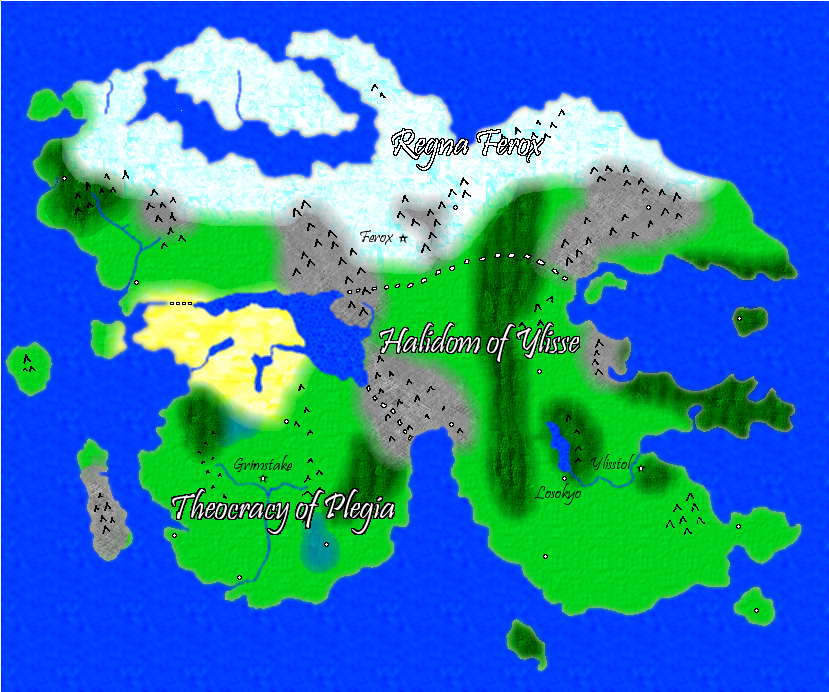
\includegraphics[scale=0.7]{archanea_colored.png}
\end{center}
\newpage
\tableofcontents
\newpage

\section{Introduction}

Fifteen years ago, in the year 63 Mostyn, the Exalt of \linkto{nations:ylisse} declared a crusade against \linkto{nations:plegia}, vowing to rid the continent of the Grimleal (followers of the dragon \linkto{religion:grima}), whom Ylissean religion deems to be evil agents of discord and destruction. However, Ylisse failed to progress very far into Plegian territory, and the war stood at a stalemate for twelve long years. It was at that point, three years ago, that the Exalt suddenly died and his daughter, \linkto{people:emmeryn}, took the throne. A compassionate ruler, Emmeryn quickly negotiated a white peace with Plegia's \linkto{people:gangrel} and focused her attention to healing the realm from the scars of war. Plegians remain skeptical of the new Exalt's compassion, and harbor deep hatred towards all Ylisseans in the wake of that war.

The \linkto{nations:ferox} to the north is a collection of kingdoms, divided in loyalty to the Eastern and Western Khanates, which are both sovereign under the Feroxi throne. In Ferox, strength is the most valued quality of all, and politics revolves around posturing oneself as stronger than the alternatives. Because of this, little attention is paid to the goings-on outside Feroxi borders, and thus Ferox is able to maintain warm relations with both Ylisse and Plegia. 

\subsection{Losokyo}

Losokyo, like any large city, has been plagued with thieves and pickpockets for time immemorial. However, soon after the Ylissean Crusade began to truly wear on the Halidom, about two years into the war, criminal elements began taking over large sections of the city. In response, the city took drastic measures to combat the crime problem and suspended the principle of ``innocent until proven guilty''. The local priestesses of \linkto{religion:themis}, the dragon of Justice, fearing their god's retribution, rapidly trained prosecutors, defense attorneys, and judges in an attempt to ensure justice is carried out even under these dire circumstances.
% nd, due to the stress this caused the legal system, enacted a maximum time limit on court cases and
\begin{center}
``The end is only justified through proper means'' \\
- Inscription on the Central Courthouse
\end{center}

The priestesses maintained this practice for a couple years, until 68 Mostyn, when they left Losokyo to establish the Themis Legal Academy in a more central location of the Halidom, in order to train legal experts for use across the realm. However, with their departure, the people of Losokyo have gradually lost faith in this new legal system, particularly becoming wary of corrupt prosecutors fabricating evidence and police incompetence. Among several events, two in particular stand out as embarrassing failures of justice.

\begin{enumerate}
\item \linkto{events:dl6}\\
During this period of prosecutorial corruption, public faith in the law rested entirely on the defense attorneys. In 73 Mostyn, one of the most famous defense attorneys, \linkto{people:gregory}, took on master prosecutor \linkto{people:mvonkarma} in a high profile case. During a recess in the trial, Gregory was in a lift with his son, \linkto{people:miles}, and a court bailiff, \linkto{people:yogi}, when an earthquake struck, incapacitating the lift for a period of time. When the lift was repaired and opened, Gregory was found dead, shot by a gun.

The police were unable to make any progress on this case, and so secretly consulted \linkto{people:mistyfey}, a spirit medium and head of \linkto{places:kurain}. Misty channeled Gregory's spirit, who fingered Yogi as the culprit. The fact that the police consulted a spirit medium was leaked to the press, causing a scandal. Further, Yogi's attorney, \linkto{people:hammond}, succeeded on acquitting his client through pleading temporary insanity. 

\item \linkto{events:kidnapdh}\\
Not too long after the DL-6 incident, \linkto{people:fawles} kidnapped \linkto{people:dahlia}, the daughter of a wealthy jeweler, and demanded a \$250,000 GP diamond for her return, to be delivered to \linkto{places:duskybridge}. \linkto{people:valerie}, Dahlia's sister and a police officer, was chosen to conduct the random payment, however Fawles pushed Dahlia off the side of the bridge midway through. Dahlia fell into the dangerous current to almost certain death, and the gem was lost as well. For this, Fawles was sentenced to death, however as of Emmeryn 2, his sentence has not been carried out.
\end{enumerate}

Under the peace brought to the halidom by Exalt \linkto{people:emmeryn}, Losokyo has seen only a slight return to order. In recent months, police have been flummoxed by a series of murders that they have been unable to solve. Outside the city, bandits terrorize merchants, who are nearly defenseless after the Exalt's downsizing of the Ylissean army. Losokyan militas have scoured the countrysides in search of bandit camps, but have made little progress. Unbeknownst to the civillians, many of these bandits are actually Plegian raiding parties, directed by \linkto{people:gangrel} in attempts to re-ignite war between Ylisse and Plegia.

\subsection{Ylisse}
Recognizing the need for her halidom to heal after the trials of the Crusade, Exalt \linkto{people:emmeryn} has turned her attention to internal affairs. She all but disbanded the Ylissean army, allowing those soldiers to return to their villages, which had suffered from a lack of manpower to tend to farms and workshops. Instead, Ylisse's internal affairs are protected by the Shepherds, a royal guard led by Prince \linkto{people:chrom} that travels across the realm to protect against bandits and other threats. While effective when present, the Shepherds are unable to protect the entire halidom at once, and bandit attacks have only grown in frequency. This, however, is also largely due to Plegian raiding parties that disguise themselves as bandits to terrorize Ylissean towns. The Shepherds are aware of the true identity of these ``bandits'', however Emmeryn is adamant in avoiding another war.

\section{The First Turnabout}
The party enters Losokyo expecting to meet \linkto{people:miafey}, however they are met by \linkto{people:starr}, who welcomes them and informs the party that Mia is busy and so they were asked to show them around. Angel Starr guides them to the center of the city, pointing out the central Court House and the clock tower at the top. 
\begin{center}
``It truly is a wonderful chime. I've lived here for nigh on a decade and still enjoy its song every hour.''
- Angel Starr \end{center}

After answering any questions the party may have about the city, Angel Starr then directs them towards the Gatewater Hotel, where rooms have already been reserved for the party. Shortly after entering, however, Angel Starr leaves the party to exit the hotel in order to hear the 4PM chime of the clock tower, inviting the party out to hear it.

\begin{center}
``This hotel is special; you can't hear the clock tower from inside. I figure they don't want it disturbing the guests if they're trying to nap midday or something. This hotel serves plenty of foreign tourists, who may suffer from tele-lag. Similarly, the rooms are entirely sound-proof.''
\end{center}

Upon re-entering the hotel, \linkto{people:larry} walks by, possibly unnoticed. If noticed, he is clearly annoyed and unwilling to talk to anyone. Angel Starr then leads the party to their room, a suite with N bedrooms on the side of a large meeting room on the fourth floor. There is a balcony, which looks over Fey \& Co. Law Offices. When the lighting is right (say, at night), you can see right through the window into the main office. Angel Starr answers any questions the party has about the accomodations and the city, and further informs them that Mia needed to defend a client in court on a very short notice, and so won't be available until later tonight.

About two hours later, if the party is in a public place, Detective \linkto{people:gumshoe} and the Losokyan police will arrive and arrest one of the party members (that looks like Larry\footnote{Setting this PC up to constantly be referred to as ``Harry Butz'' for the next week or so} for murder, and take that member to the Detention Center, and the trial will be tomorrow. Alternatively, if Larry is a close friend of any of the party members, he will be arrested instead. If the party figures out the crime scene and attempts to investigate it, they will mostly be stonewalled, as they are not lawyers and thus aren't allowed to investigate. However they might learn the following information from talking to Detective Gumshoe:
\begin{itemize}
\item The victim's name was Cindy Stone
\item Cindy was murdered via blunt force trauma
\item Cindy had just returned from Babahl
\end{itemize}
In particular, if the party asks anyone about Babahl, they should mention the need to change clocks.
\begin{center}
``Babahl? I've heard that place is wonderful, really well suited for tourists. There's just one annoyance, which is that it's so far away you have to adjust your clocks like nine hours ahead. Really messes with your system, you know?''
\end{center}

If the party goes to the detention center and the suspect is Larry, he will be confused. Earlier that day he went to Gatewater Hotel to visit his girlfriend, but she wasn't home, so he left and wandered around for the rest of the day. If pressed, he will say his girlfriend's name is Cindy Stone. If he finds out that Cindy Stone was murdered, he goes insane, blabbering about how his life is over, nothing matters anymore, he might as well get a guilty verdict, etc. 

\begin{center}
``Oh, it's all over... I... I'm finished. Finished! I can't live in a world without her! I can't! Who... who took her away from me? Who did this!? Aww, ya gotta tell me! Who took my baby away!?''
\end{center}

At some point, the party will be asked who will be defending the suspect. The only acceptable answer is for the party themselves (or a subset thereof) to do the defense, as they will not be able to meet with Mia before the deadline, and no lawyers they may find will be willing to take on a client with such short notice.

That night, Mia will visit the party and tell them she heard about what happened (if the suspect is not Larry), and asks if they managed to find a lawyer. Since the party has already registered themselves as the defense, Mia won't be able to be the attorney, however she will offer to stand at the bench as an assistant. 

\subsection{Trial}
The trial begins at 10 AM, although the group and the defendant meet in Defendant Lobby No. 2 to prepare for the case. If Larry was not the culprit, the bailiff will approach the party and inform them that due to new, conclusive evidence, the suspect in this case is now Larry Butz. Larry pleads with the party to save him, and Mia encourages the party to continue the defense, as he doesn't seem guilty. Once they have agreed, however, Larry will become incoherent, and the group continues discussing the case until the trial begins. Either Mia or the Bailiff will bring the party \linkto{evidence:cindyautopsy}. In the Courtroom, the \linkto{people:judge} will note that the defense team is new, and give a short test to ascertain their readiness:
\begin{itemize}
\item Please state the name of the defendant in this case. (If multiple choice: Party Member, Larry Butz, Mia Fey)
\item This is a murder trial; tell me, what wsa the victim's name? (If multiple choice: Mia Fey, Cinder Block, Cindy Stone)
\item What was the cause of death? She died because she was... (If multiple choice: Poisoned, hit with a blunt object, strangled)
\end{itemize}

The Judge then invites the prosecutor, \linkto{people:wpayne}, to explain what the murder weapon was: \linkto{evidence:thinker}, found lying on the floor, next to the victim. The prosecutor then calls Larry to the stand and asks some questions.

\subsubsection{Witness Testimony: Larry Butz}
\begin{center}
\begin{tabular}{p{2.5in} p{2.5in}}
Mr. Payne & Larry \\\hline
Ahem, Mr. Butz. Is it not true that the victim had recently dumped you? & Hey, watch it buddy! We were great together! We were Romeo and Juliet, Cleopatra and Mark Anthony! I wasn't dumped! She just wasn't responding to any of my letters! Or seeing me.. Ever. WHAT'S IT TO YOU, ANYWAY!? (continue from transcript, until ``Duuude!'')\\
We can clearly see what kind of woman this Ms. Stone was. Tell me, Mr. Butz, what do you think of her now? \\
\end{tabular}
\end{center}

At this point, Mia turns to the party and tells them that it would probably not be good to let Larry answer that question, although whether the party lets him or not, he will. Additionally, during that line of questioning, Payne will introduce the victim's \linkto{evidence:passport}, as evidence the victim went to Babahl.


\begin{center}
\begin{tabular}{p{2.5in} p{2.5in}}
Mr. Payne & Larry \\\hline
I believe the accused's motive is clear to everyone. Next queston! You went to the victim's apartment on the day of the murder, did you not? & Heh? Heh heh. Well, maybe I did, and maybe I didn't!
\end{tabular}
\end{center}

The Judge turns to the party, asking them to advise their client to answer the question. Regardless of whether they do, Mr. Payne interjects that he has a witness proving Larry did go to the victim's apartment that day. 

\begin{center}
``On the day of the murder, my witness was selling newspapers at the victim's building. Please bring Mr. Frank Sahwit to the stand!''
\end{center}

\subsubsection{Witness Testimony: Frank Sahwit 1}
\begin{center}
\begin{tabular}{p{4in}}
I was going door-to-door, selling subscriptions when I saw a man fleeing an apartment.\\
I thought he must be in a hurry because he left the door half-open behind him. \\
Thinking it strange, I looked inside the apartment. Then I saw her lying there... A woman... not moving... dead! \\
I quailed in fright and found myself unable to go inside. \\
I left to notify the police immediately! \\
I went to a nearby park and found a patrolling officer. \\
I remember the time exactly: It was 11:00 AM. \\
The man who ran was, without a doubt, the defendant sitting right over there. \\
\end{tabular}
\end{center}

Once the statement is over, the Judge asks Mr. Payne why the witness had to go all the way to a park to find a police officer, to which Mr. Payne informs the Judge that the same enchantments used to mute the clock tower occasionally disrupt police communications, and so they prefer not to patrol near the hotel. Satisfied, the Judge allows the party to begin their cross-examination. Mia, excited, tells the party that this is their chance to expose the lies in the witness's statement, and gives an introduction to the courtroom mechanics.

\begin{center}
``First, find contradictions between the evidence and the witness's testimony. Then, once you've found the contradicting evidence... present it and rub it in the witness's face!''
\end{center}

The contradiction is between the reported time (11:00 AM) and the time of death in the autopsy report (around 2-3 PM). While Payne tries to claim that the witness merely forgot the time, the Judge disagrees that that was possible, given how certain Sahwit was. After some discussion, Sahwit realizes what happens and asks to give further testimony.

\subsubsection{Witness Testimony: Frank Sahwit 2}
\begin{center}
\begin{tabular}{p{4in}}
You see, when I found the body, I heard the time. \\
There was a voice saying the time... It was probably coming from a neighboring room \\
Oh, but it was three hours off, wasn't it? \\
I guess the neighbors must have been discussing the past! \\
That's why I thought it was 11:00 AM! \\
Terribly sorry about the misunderstanding...
\end{tabular}
\end{center}

The contradiction is that rooms at the Gatewater Hotel are soundproof, and so it was impossible for someone to have heard a conversation coming from another room. Sahwit, increasingly agitated, comes up with another explanation, although the Judge is starting to become frustrated with the frequent corrections. \\

\subsubsection{Witness Testimony: Frank Sahwit 3}
\begin{center}
\begin{tabular}{p{4in}}
Actually, I didn't ``hear'' the time... I ``saw'' it!\\
There was a table clock in the apartment, wasn't there!\\
Yeah, the murder weapon! The killer used it to hit the victim!\\
That must have been what I saw. \\
\end{tabular}\end{center}

The contradiction is that the murder weapon was a statue, not a clock. Sahwit is starting to get angry and defensive now,\\
\begin{center}
``Whaa!? Y-you with your ``objections'', and your ``evidence''... Just who do you think you are!? Hey, I... I saw it there okay! That's a clock!''
\end{center}
At this point, Payne interrupts and informs the court that the statue is in fact a clock, that tells the time out loud when its neck is turned. However, since it looks like a statue, he submitted it as a statue. This, however, does not clarify how Sahwit knew it was a clock. The only reasonable explanation is that Sahwit went inside the apartment, and thus is likely the murderer. Sahwit is now almost incomprehensible.\\
\begin{center}
``I... I...! That... that day... I... I never! Look... I... the clock... I heard, no! I mean, I saw...Saw...nggg! Gwaaaaaah! Shutupshutupshutup! I hate you! I-it was him, I tell you! I saw him! H-he killed her and he should burn! Burn! Give him death!''\\
Frank then throws his toupee at a party member (DC 12 DEX save)
=\end{center}
After a moment of shock after his outburst, Payne steps up, flustered, pleading with the Judge not to be hasty, as there is not any evidence supporting the defense's claims. In response, the Judge asks the defense if they have any evidence that the sound the witness heard came from the clock. The only allowed response is to sound the clock; other options either have Mia butt in and explain why that is a bad idea, or the Judge will explain and penalize the party. \\
\begin{center}
``...*beep*...\textit{I think it's 8:25}''
\end{center}
The current time, of course, is 11:25. While this seems incriminating, Sahwit objects, saying that it proves nothing, as you have no way of showing that the clock was running slow on the day of the murder. The Judge, concurring, says that due to the lack of evidence, the cross-examination of Mr. Sahwit is over. If the party doesn't realize that they can prove the clock was running slow because it is still running on Babahlese time, Mia will object.
\begin{center}
``Don't waste time doubting the facts. Assume the clock was three hours slow and... Think through it! Ask yourself, `Why was the clock three hours slow?' Figure out the reason, and you'll have your proof! Right? Can you think of a reason as to why the clock would be three hours slow?''\end{center}
Satisfied, the Judge orders the arrest of Mr. Sahwit, and compliments the defense on such a quick case and on finding the true culprit. After some more possible pleasantries, he delivers his verdict: Not Guilty. 

\subsection{Post-Trial}

Mia congratulates the team on a job well done, but the cheery mood is spoiled by Larry's moping about his dead girlfriend. Mia congratulates ``Harry'', and after some conversation, gives a \linkto{items:thinker} to both Mia and to the party, although the one for the party looks a little wonky. He made three; one for Cindy and one for him, and one for practice. He then comments that he can't believe Cindy was playing him for a fool, that he was just another of her men. Mia disagrees, saying that she thinks that Cindy actually did have feelings for him, and prompts the party to explain what she's talking about. She is referring to the Thinker Statue, which Cindy took with her to Babahl, despite its bulk. If the party gives the wrong explanation, Larry will see through it, but in either case thank everyone and walk off. 

\begin{center}
``I hope you see the importance of evidence now. Also, hopefully you realize, things change depending on how you look at them. People, too. We never really know if our clients are guilty or innocent. All we can do is believe in them. And in order to believe in them, you have to believe in yourself. Listen. Learn. Grow strong. Never let go of what you believe in. Never.''\end{center}

Mia then will invite the party to dinner on her, toasting to ``an innocent Butz''.
\qed

\subsection{Evidence}
\subsubsection{Cindy's Autopsy Report}
\label{evidence:cindyautopsy}
Time of death: 2-3 PM, Ket 21. Cause of death: loss of blood due to blunt force trauma. 


\subsubsection{Thinker Statue}
\label{evidence:thinker}
A statue in the shape of ``The Thinker''. It's rather heavy. See \linkto{items:thinker}.

\subsubsection{Passport}
\label{evidence:passport}
Cindy Stone apparently returned from Babahl on Ket 20, the day before the murder. 


\section{Religion}
\subsection{Dragon gods}
\subsubsection{Anankos}
\label{religion:anankos}

\subsubsection{Eitri}
\label{religion:eitri}
Ancient divine dragon of artisans. Has a sect in Losokyo that practices black magic.

\subsubsection{Grima}
\label{religion:grima}

\subsubsection{Naga}
\label{religion:naga}

\subsubsection{Themis}
\label{religion:themis}


\section{People}
\subsection{Plegia}


\subsubsection{Broderick}
\label{people:tslil}
\begin{center}
\begin{tabular}{c c|c c}
STR & 13 & INT & 9\\
DEX & 18 & WIS & 16 \\
CON & 12 & CHA & 9 \end{tabular}\end{center}
\textit{Human Monk}\\
A fellblood bearing the Mark of Grima on the back of their right hand. Son of \linkto{people:validar} and Lide, he bears both the proper Heart and Blood of Grima to be the Fell Dragon's vessel and aid in its ressurection. Unwilling to sacrifice her son for this purpose, Lide took Broderick and fled to Ylisse on his tenth birthday. For their protection, she disguised herself as a relative, Aunt Milibette, and told Broderick that his parents were killed. When Broderick was 15, \linkto{religion:grima}, through the time travel process initiated by \linkto{people:bends} and \linkto{religion:naga}, attempted to take control of his body, however Broderick was too weak and instead lost all of his memories and gained the Mark, occasionally receiving visions of Grima's future. Lide, alarmed by the appearance of the Mark, gave him an earring, \linkto{items:lideearring}, to hide it. However, when Broderick reveals his visions to her, she realizes that he is not safe with her and leaves him in the care of the nearby monastery.

Broderick's childhood is as much a mystery now, to him, as it has ever
been. Beyond fleeting and shattered fragments of jagged rememberings,
none quite seeming real or ever lingering long enough to be processed
by the conscious mind, Broderick would not be able to describe the
circumstances of his youth any more than he would be able to explain
how he came to be in the care of his aunt Milibette. As far as he is
concerned, things have roughly always been this way.

For as far back as contiguous or even tangible memory extends,
Broderick had lived in a small hut with Hilda, nestled in the
foothills of a mountain where they tended to their meagre fields and
few livestock, all but isolated from the world. A day's journey in one
direction lead to a village too insignificant for even for the most
detailed of maps, a village of no particular import and of no
particular name. A few day's journey in another direction, up the
mountain lead to a monastery. It was for this monastery, the Monastery
of Highsleaux, and the mountain Ebpel Rulugenpud as the monks
insisted, that Milibette had brought Broderick here.

His story, as she would he had it, was that Broderick was once son to
a loving father and mother. Agen and Lide were their names, and they
cared for their son without thought for another. Through stout labour
and husbandry they ensured that all the needs of young Broderick were
met, and Agen was a skilled carpenter out of whose workshop many a toy
were produced. There, Milibette said, was were Broderick honed his
keen senses in the careful measuring and alignment of the structures
his father built, and the warding of the fields from small game. Life
was bliss, she said, but as is the capricious nature of the gods this
joy was torn maliciously from its stem before a flower it could
become, and the soil sown with the unspeakable crimes that it
witnessed.

Milibette spoke sparingly of this terminal frost, a marauding group of
Orcs attacked the village to which the homestead was adjoined,
methodically and deliberately paring all that had been brought to
blossom. She was taking care of Broderick while Agen and Lide were out
trading wares with the villagers. The orcs raided the home on their
way out, while the child and guardian quivered silently in the barn.

More of these events Broderick would never learn, and even such scant
recollections were hard to come by -- Milibette only hinting at them
on rare evenings during which some inner force of irreconcilable guilt
or sadness seemed to be consuming her. The same forces, she asserted,
held Brodericks memories captive -- unwilling to relinquish their icy
grasp lest Broderick's very person be rended asunder by the horrid
truth. Trauma, it would seem, was both an agent of terrible change and
one of sterilisation. The wound was unfathomably deep, but clean.

All of this was why the had to move. She collected what remained,
spared no comfort, and attempted to replant far away from all of this,
in the safety of anonymity and insignificance, under the careful watch
of the monks. And so Broderick came to be, again. The only hint that
any of this was real, aside from the yawning cavity in his memories,
was a simple earring. An earring, Milibette said, which had belonged
to Lide -- whoever she was.

Broderick would have let this all be, put it aside to the best of his
abilities, were it not for the visions. They came, infrequently at
first, manifesting as headaches before some transplanting of reality
occurred so believable that Broderick could scarcely reconnect with
the world upon their termination. He dared not speak of them for many
years, and when he finally did, his world was once more torn from its
roots.

Milibette announced that he was to be deposited in the care of the
monks, she could no longer tend to him and he would not flourish under
her care. He had barely organised his reality when he was forced into
a life of asceticism and study. Milibette moved to the village, but
Broderick was not permitted to leave the extended grounds of the
monastery all to visit her.

Many years passed in the monastery << more here >> but he never quite
seemed to grow in the way they wanted. Books had their uses, he
admitted, but he would often choose to spend his time alone, away, on
the outskirts of the grounds, testing his eyes against the landscape
as though one day they might be trained to become sharp enough to
finally notice the flaw in reality -- the seem at the very edge of the
world that would reveal to him what was behind it all. He lived to
perceive, and hoped that one day he would have the clarity to pierce
the miasma clouding his memories or the strangling darkness obscuring
his visions. One day he would be able to look upon his life and see,
see who he was and what it was all for.

\subsubsection{King Gangrel}
\label{people:gangrel}

\subsubsection{Validar}
\label{people:validar}
A human illusionist and head of the Grimleal. Years of religious loyalty to Grima and practice of dark magic has twisted his form, and so he now permanently dons an illusion to look like a tiefling to mask his horrid figure. The source of this illusion is his holy symbol, a \linkto{items:grimanecklace}, which he always wears under his cloak.

\subsection{Regna Ferox}

\subsubsection{Klob Rockbeard}
\label{people:daniel}
\begin{center}
\begin{tabular}{c c|c c}
STR & 18 & INT & 8\\
DEX & 14 & WIS & 10 \\
CON & 19 & CHA & 10 \end{tabular}\end{center}
\textit{Dwarf Barbarian}\\


\subsection{Ylisse}

\subsubsection{Aleneth}
\label{people:bends}
\begin{center}
\begin{tabular}{c c|c c}
STR & 10 & INT & 14\\
DEX & 12 & WIS & 9 \\
CON & 14 & CHA & 20 \end{tabular}\end{center}
\textit{Half-elf Warlock}\\

Identity taken of Exalt Lucina in order to disguise her presence in the current timeline. The daughter of Krom and ??? ten years from the start of the campaign, she became Exalt after the death of her mother, which immediately preceded the rebirth of \linkto{religion:grima}. With her world's destruction at hand, she and her companions manage to recover all but one of the gems (Argent) and perform the Awakening ritual. However, without the full complement of gemstones, \linkto{religion:naga} is unable to impart her full power to the \linkto{items:falchion}, instead sending Lucina and her companions back in time to shortly before the start of the campaign. 

Unbeknownst to Lucina, Grima interferes with this process, causing the travellers to all arrive in different times and locations, and attempts to take control of his vessel, \linkto{people:tslil}. However, Broderick's body is too weak to hold all of Grima's power, and instead he loses his memory and gains the Mark of Grima. Grima also created another timeline, initially without Naga's knowledge. 
\begin{itemize}
\item If Grima is sealed away in both timelines, then so too will he be sealed in the ``true'' timeline, as the three paths work to recombine. Lucina and the others will be allowed to return to their timeline.
\begin{itemize}
\item In this case, if Grima is \textit{killed} in either timeline, he will be killed in all of them
\end{itemize}
\item If Grima is awakened in both timelines and allowed to reach full strength, then Lucina and the party will be unable to return to their timline, and all will be lost.
\item If Grima is only sealed in one timeline, then Lucina and the party will be able to return to their timeline, however the events in the two timelines may have altered the state of affairs
\end{itemize}

Because the Awakening was performed without all the gemstones, Lucina also needed to offer her right hand as sacrifice, replacing some of the power of the missing gemstone, Argent. She has three main goals that she needs to accomplish in order to hopefully prevent the ressurection of Grima:
\begin{enumerate}
\item Prevent an assassination attempt on Krom, which later leads to his death
\item Prevent the assassination of Exalt Emmeryn
\item Prevent Plegia from obtaining the Shield of Seals and the gemstones.
\end{enumerate}

Lucina knows that her mother was killed by someone close to her, but does not know it was actually \linkto{people:tslil}.

\subsubsection{April May}
\label{people:aprilmay}
\begin{center}
\begin{tabular}{c c|c c}
STR & 8 & INT & 11\\
DEX & 15 & WIS & 11 \\
CON & 11 & CHA & 17 \end{tabular}\end{center}
\textit{Human}\\

\subsubsection{Bucky Whet}
\label{people:bucky}
Son of Farina Whet, ``Whet Noodle No. 3'' and head soba chef at the Whet Noodle. 


\subsubsection{Dahlia Hawthorne}
\label{people:dahlia}

\subsubsection{Dick Gumshoe}
\label{people:gumshoe}
\begin{center}
\begin{tabular}{c c|c c}
STR & 15 & INT & 6\\
DEX & 9 & WIS & 6 \\
CON & 16 & CHA & 11 \end{tabular}\end{center}
\textit{Human}\\

\subsubsection{Emmeryn}
\label{people:emmeryn}

\subsubsection{Gilbert Wright}
\label{people:phoenix}
\begin{center}
\begin{tabular}{c c|c c}
STR & 13 & INT & 11\\
DEX & 17 & WIS & 12 \\
CON & 13 & CHA & 14 \end{tabular}\end{center}
\textit{Human}\\
A literature student at Ivy University, and former ``boyfriend'' of \linkto{people:dahlia}. 

\subsubsection{Gregory Edgeworth}
\label{people:gregory}

\subsubsection{Judge}
\label{people:judge}


\subsubsection{Krom}
\label{people:chrom}



\subsubsection{Larry Butz}
\label{people:larry}
\begin{center}
\begin{tabular}{c c|c c}
STR & 11 & INT & 7\\
DEX & 14 & WIS & 6 \\
CON & 10 & CHA & 14 \end{tabular}\end{center}
\textit{Human}\\
Originally from the same gaucho community as \linkto{people:david}, Larry and San Juro were close childhood friends until Larry's family moved to Losokyo in 65 Mostyn. Notoriously excitable and lazy, he was infamous for getting caught up in unfortunate situations, to the point where a saying developed: ``When something smells, it's usually the Butz''. At the start of the campaign, Larry is dating Cindy Stone, a model.

\subsubsection{Manfred von Karma}
\label{people:mvonkarma}

\subsubsection{Maya Fey}
\label{people:mayafey}

\subsubsection{Miles Edgeworth}
\label{people:miles}

\subsubsection{Mia Fey}
\label{people:miafey}
\begin{center}
\begin{tabular}{c c|c c}
STR & 9 & INT & 17\\
DEX & 12 & WIS & 15 \\
CON & 11 & CHA & 16 \end{tabular}\end{center}
\textit{Human}\\



\subsubsection{Misty Fey}
\label{people:mistyfey}

\subsubsection{Mr. Briney}
\label{people:mrbriney}
\begin{center}
\begin{tabular}{c c|c c}
STR & 12 & INT & 17\\
DEX & 10 & WIS & 17 \\
CON & 12 & CHA & 14 \end{tabular}\end{center}
\textit{Human}\\
An old sailor living on the shore of Yam Lake with a seagull named Peeko. His wife, Calliope, was a sorceress who died during the Crusade. Before she left for the war, she crafted a figurine of a seagull (\linkto{items:peeko}) using driftwood near their cottage and bound her familiar to it as a gift to her husband so that a part of her would always remain by his side during the war. With her death, Peeko is Mr. Briney's only memento of his wife, but tragically the statuette was stolen by bandits a couple weeks before the campaign began (early Ket). 


\subsubsection{Norric}
\label{people:jeff}
\begin{center}
\begin{tabular}{c c|c c}
STR & 18 & INT & 11\\
DEX & 14 & WIS & 18 \\
CON & 13 & CHA & 13 \end{tabular}\end{center}
\textit{Wood Elf Druid, Circle of Land}\\

Born under the childhood name Nor in a small village of wood elves, on the outskirts of a forest some number of miles from the Ylissean city of Losokyo, this druid developed a natural attunement with nature in his early years. Nor played with the tiny critters of the forest almost as often as his fellow elves, and more than once stared at a watchful wolf with mere curiosity before the predator reconsidered its next meal. Distanced from danger on account of his innate interaction with beasts, Nor spend the later years of his childhood roaming the inner portions of the forest, discovering on his own an ability to cure animals of their wounds through extraordinary talent. 

Once, when the seasonal rains bore down upon the forest and Nor was far too deep into the forest to safely return home, far too cold to survive through mundane means, he channeled a flame upon his palm to his own wide astonishment. Perhaps it was the call from Nature that had led Nor to the front doorstep of a circle of druids so that they may have witnessed this event - but as Nor soon realized, these guardians of the woods had sensed Nor's talent for many years, and welcomed his presence. After several years of careful guidance with these masters of the wilderness, Nor returned from the heart of the forest under his new adult name, Norric. His craft for healing cultivated and his call to defend Nature fully manifested, Norric soon discovered that the meager workings of the wood elf village in which he was raised, the inhabitants of which so aloof from both the beauties of the forest and the majesties of the outside world, were inadequate. How were these elves so far removed from Nature? Why did they not see a need to better the beautiful world around them? 

Norric, who had yet to venture further than the forest outskirt's, was unaware that the elves had so secluded themselves on account of the political dangers surrouding them - dangers of which Norric has so far lived in ignorance. His outlook in life, that all of the world is a manifestation of Nature and can be mended with proper effort, will surely be put to the test as he leave his village, this time away from the forest; what more, Norric's short life as a wood elf and as a druid has secluded him from the very society he now ventures to "cure", and will surely contrast with his expert use of divine, wild ability.

\subsubsection{Redd White}
\label{people:redd}
\begin{center}
\begin{tabular}{c c|c c}
STR & 12 & INT & 8 \\
DEX & 15 & WIS & 12 \\
CON & 12 & CHA & 20 \end{tabular}\end{center}
\textit{Human}\\
Currently the CEO of the information-gathering company Bluecorp, a company that works on projects ranging from detective work to journalism to foreign intelligence. However, all of Bluecorp's activities are with the aim of uncovering kompromat on individuals for the purposes of blackmail, a project that has been remarkably successful and makes Bluecorp, and by extension, Redd, all but untouchable by the law. \\
\\
While not a member of the Grimleal, Redd White was approached by the Grimleal during the Crusade to sell information to the Plegians in order to hamper the Ylisseans. While some contact is still maintained, Redd and his company currently work mostly independently from Plegia. \\
\\
One of Bluecorp's early successes outside of anti-Crusade work was the acquisition of the secret behind \linkto{events:dl6}, which it bought from \linkto{people:grossberg} and subsequently leaked to the media. This won him control over Grossberg as the police began to search for the source of the leak.\\
\\
Bluecorp employs a great number of people to perform its information gathering. These include his secretary \linkto{people:aprilmay}, a bandit captain Stella Artois, and close associate Himika Kazuro (\linkto{people:cyew}). \\
\\
A rather pompous man, Redd frequently makes up his own words or switches into Spanish. He collects magical artifacts, a hobby financed by his lucrative business. As such, he very well protected with warded items, and nearly unbeatable when on his own turf. 

\subsubsection{Robert Hammond}
\label{people:hammond}

\subsubsection{San Juro}
\label{people:david}
\begin{center}
\begin{tabular}{c c|c c}
STR & 9 & INT & 9 \\
DEX & 19 & WIS & 15 \\
CON & 12 & CHA & 14 \end{tabular}\end{center}
\textit{Human Gunslinger}\\
\\
San Juro was a gaucho in the southern planes, part of a small bison wrangling community. His wife was due with child. Due to the dangers of the wild, and the threats of bandit raids, he always carried his trusty pistol at his side. He lived a simple life until one day, a raid by the notorious Five Fists bandit crew upended everything. The crew shot his wife dead as they ransacked the town, and San swore revenge. Having shot a lackey dead, he picked up his pistol (begining his dual wielding trend), and tracked down the rest of the crew.

When he found them, however, they had already got got, and were lying bleeding or dead by the roadside. Before finishing off the wounded, San found that one of the crew had ran. Broken and defeated by his unfinished revenge, San became a hired gun, roaming the southern planes and the towns therein.


\subsubsection{Terry Fawles}
\label{people:fawles}

\subsubsection{Thalassa Gramarye}
\label{people:thalassa}

\subsubsection{Valerie Hawthorne}
\label{people:valerie}

\subsubsection{Winston Payne}
\label{people:wpayne}


\subsubsection{Yanni Yogi}
\label{people:yogi}

\section{Places}

\subsection{Borginia}
\label{nations:borginia}

\subsection{Cohdopia}
\label{nations:cohdopia}
Split into two nations, Allebahst and Babahl, in Naga 1002, 

\subsubsection{Allebahst}
\label{nations:allebahst}
\subsubsection{Cohdopian Normal School}
\label{places:cns}
Unlike the \linkto{places:arcaneinstitute}, the Cohdopian Normal School produces items in which magic is only a supporting element, if it exists at all. While neither school really produces weapons, an alumnus of CNS, Cole Grande, was the first to construct a gun some 75 years ago, which has been refined ever since to the variety of guns we have today. Further, while the Institute's magic is primarily of the \textit{evocation} and \textit{illusion} schools, the CNS largely specializes in \textit{transmutation} and \textit{abjuration}.
\subsubsection{Babahl}
\label{nations:babahl}
National symbol is a butterfly, called a ``H\=ato''.

\subsection{Plegia}
\label{nations:plegia}

\subsubsection{Grimstake}
\label{places:grimstake}

\subsection{Regna Ferox}
\label{nations:ferox}

\subsubsection{Ferox}
\label{places:ferox}

\subsection{Ylisse}
\label{nations:ylisse}

\subsubsection{Arcane Institute}
\label{places:arcaneinstitute}
The gem of Ivy University and central to the Losokyan way of life, the Arcane Institute develops items that allow everyone to benefit from the conveniences of magic. Some of the Institute's most famous inventions include
\begin{itemize}
\item Sender blocks and the Red network, which allow for instantaneous communication for any two people within the network\\
The price of a sender block depends on its charge capacity and recharge rate, typically
\[ price = 3 * capacity + 2*recharge \]
The most common models are the (1,1d1) for 5gp, (5,1d4) for 20gp, (10,1d6) for 35gp, and (20,3d6) for 80 gp. 
\item Lights\\
These come in various sizes, intensities, and colors, although their price increases the further from ``baseball-sized 20' range white''. These also require \textit{serifs} from a magic font to run. Many buildings run a connection to the main font in the Institute, but portable fonts and font generators are also available.
\item Portable fonts, which are organized into how much \textit{serifs} they contain. In increasing volume, the primary sizes are ``Q'', ``V'', ``N'', and ``F''. 
\item Cameras, onamonapoetically called ``Shashin''; these print their pictures after a short delay (think polaroid)
\item \st{Action} Video cameras, however they can typically only record in greyscale and require \textit{serifs} to run.
\end{itemize}

\subsubsection{Eagle Mountains}
\label{places:eaglemountains}
A mountain range opposite Losokyo on Yam Lake. Home to Hazakura Temple and Dusky Bridge, however it has been mostly abandoned since the ``murder'' of Dahlia Hawthorne, with one notable exception being the murder of Valerie Hawthorne. Because of this, while the road to Dusky Bridge is still followable, the area away from the temple is still fairly wild, with a base 20\% chance of encountering hostile wildlife during a given period of time. Beyond the temple, the mountains are much more untamed, with a base 40\% chance of encounter.  In such an instance, roll a d20 to determine what appears:\\
\begin{center}
\begin{tabular}{c c c}
Roll & Outskirts & Heart \\\hline
1 & Swarm of Poisonous Snakes  & Goblin party \\
2-5 & Dire wolves & Black Bears \\
6-10 & Black Bears & Giant Insects \\
11-15 & Giant insects & Swarm of Ravens \\
16-20 & Swarm of Bats  & Swarm of Insects \end{tabular}\end{center}

\subsubsection{Dusky Bridge}
\label{places:duskybridge}

\subsubsection{Kurain Village}
\label{places:kurain}

\subsubsection{Losokyo}
\label{places:losokyo}
A large city on Gourd Lake that serves as a trade connection between the interior of Ylisse and the ocean and capital, \linkto{places:ylisstol}. 

\subsubsection{Ylisstol}
\label{places:ylisstol}

\subsection{Zheng Fa}
\label{nations:zhengfa}

\section{Events}
\subsection{The DL-6 Incident}
\label{events:dl6}


\subsection{Kidnapping of Dahlia Hawthorne}
\label{events:kidnapdh}

\subsection{The Black Canyon Conjunto}
\label{events:bcc}
A thousand years ago, when Grima first attempted to destroy the world, the two major continents of the world were united under one rule: the Empire of Archanea. The Emperor, Primidux, brought together the finest men and women of the Empire to combat this threat:\\
\begin{tabular}{c c|c c}
Sabeline & Cohdopia & Yorya & Zheng Fa \\
Durgano & Ferox & Cacto & Ferox \\
Buckeye Ro & Ylisse & Thubberd & Cohdopia\\
Burvanen & Borginia & Wayreen & Ylisse\\
Dowell & Cohdopia & Bell & Cohdopia \\
Mosto & Ylisse & Hillinnian & Ferox\\
Ischul & Ferox & Shir  & Cohdopia \\
Melbacke & Nestra & Rosegard Lyne & Ylisse \\
Bethany & Cohdopia & Validar & Plegia \\
Glen & Ylisse & Pinnick & Cohdopia\\
Nor & Ferox & ``Happy'' Val & Ferox \\
Dunlap & Cohdopia & Jomax & Ylisse \\
\end{tabular}\\

Sorted by origin:\\
\begin{minipage}[l]{0.5\textwidth}
\begin{itemize}
\item Ylisse
\begin{itemize}
\item Buckeye Ro
\item Mosto
\item Glen
\item Wayreen
\item Rosegard Lyne
\item Jomax
\end{itemize}
\item Ferox
\begin{itemize}
\item Durgano
\item Ischul
\item Nor
\item Cacto
\item Hillinnian
\item ``Happy'' Val
\end{itemize}
\end{itemize}
\end{minipage}
\begin{minipage}[r]{0.5\textwidth}
\begin{itemize}
\item Cohdopia
\begin{itemize}
\item Primidux
\item Sabeline
\item Dowell
\item Bethany
\item Dunlap
\item Thubberd
\item Shir
\item Pinnick
\end{itemize}
\item Other
\begin{itemize}
\item Plegia - Validar
\item Borginia - Burvanen
\item Nestra - Melbacke
\item Zheng Fa - Yorya
\end{itemize}
\end{itemize}
\end{minipage}
Important lore:
\begin{itemize}
\item Mosto
Mosto was an \textit{elven cleric} of Naga and the one who managed to perform the Awakening rite and seal away Grima. In recognition, Mosto rose to great fame in the Ylissean region, and after the Schism, became the First Exalt of Ylisse. Exalt Mostyn, the predecessor of Exalt Emmeryn, is named after Mosto.

\item Melbacke
Melbacke was the finest Nestri \textit{bard}, specializing in singing and dancing.

\item Validar
Validar was a \textit{human wizard} and strong ally of the Conjunto. However, as Grima was sealed away, he managed to impart some of his life force into Validar, creating a vessel to support him when he rose again. Sly-tongued, as the Shield of Seals was disassembled, he convinced the Cabinet to entrust him with the gemstone Sable, which he hid to ensure the Awakening ritual could not be performed again.

\item Primidux
Primidux became a national hero in Cohdopia, and after his death a gold statue was created to symbolize the might of Cohdopia. In the intervening years, this statue evolved into a symbol of Cohdopia itself, alonside the butterfly H\=ato and the flower Farasha. Currently, Cohdopia is split into Babahl and Allebast, and both nations hold what they believe to be the real Primidux Statue.
\end{itemize}

\section{Items}
\subsection{Babahlese Ink}
\label{items:ink}
A vial of the special ink from Babahl. Burns with distinctive green flames. Provides advantage on skill checks when used to forge documents or conterfeit currency, and reduces the cost of copying spells by 10gp per level. This vial contains enough ink for 10 pages of documents, 10 levels of spells, or 50 bills.

\subsection{Cupboard of Storing}
\label{items:cupboard}
This worn brass door knob has a dimly glowing letter C on its circular face.


Holding the door knob in the air, as if holding one belonging to a real door, a shimmering door projects in the direction the knob is pointing. Turning the handle and opening the door will reveal a cupboard with 10 shelves. At any one time, 5 shelves can be seen, only being moved by use of a pulley found inside the cupboard.


Each shelf is 4 feet wide, 1.5 feet deep, and has 2 feet of free space above it. A shelf's weight capacity is 100lb's and exceeding this will cause the shelf to disappear, tossing the contents of the shelf on to the floor.


If the Brass Knob is attached to a wall, or a real door, it is inert until removed.


Placing a Brass Knob inside an extra dimensional space created by a Bag of Holding, Portable Hole, or similar item instantly destroys both items and opens a gate to the Astral Plane. The gate originates where the one item was placed inside the other. Any creature within 10 feet of the gate is sucked through it to a random location on the Astral Plane. The gate then closes. The gate is one-way only and can't be reopened.
%https://www.reddit.com/r/DMAcademy/comments/9hzbpu/a_brass_door_knob_an_alternative_to_the_bag_of/

\subsection{Emblem of Mini/Buckle of Wumbo}
\label{items:wumbo}
A magical item in the shape of a letter ``M'', made of basalt. Contains 1 charge each of \textit{reduce} and \textit{enlarge}, which are cast by holding the item so that it looks like an ``M'' for \textit{reduce}, and upside down (``W'') for \textit{enlarge}. Casting \textit{identify} on this artifact reveals only half of its properties, corresponding to the orientation of the object. Each charge has a 25\% chance of recharging each dawn.

\subsection{Falchion}
\label{items:falchion}
A greatsword that together with the \linkto{items:fireemblem} are the Ylissean royal treasures. Forged from one of  \linkto{religion:naga}'s fangs, the sword can be empowered through the \linkto{spells:awakening} ritual.

\subsection{Figurine of Wonderous Power (seagull)}
\label{items:peeko}
A statuette of a seagull, carved out of driftwood. Acts as a normal \textit{Figurine of Wonderous Power}, and when used allows the user to cast \textit{Animal Messenger} on it. The creature contained in the figurine is a \textit{fey} seagull, previously the familiar of a now-dead Sorceress that was bound to the figurine when it was passed to the widower (\linkto{people:mrbriney}). As such, the seagull, Peeko, is primarily interested in returning to Mr. Briney, however she will still follow the commands of the owner of the figurine.\\
\\
When used by Mr. Briney, the seagull may exist in physical form indefinitely.

\subsection{Honeycomb necklace}
\label{items:honeycomb}
A \textit{cursed} necklace with a small piece of honeycomb attached. When worn, gives wearer disadvantage on all checks involving items containing the letter ``B'', and if their armor contains the letter ``B'', attacks against them have advantage. 


\subsection{Lide's Earring}
\label{items:lideearring}
A \textit{magic} earring given to \linkto{people:tslil} that, through \textit{Disguise Self}, conceals his Mark of Grima on his right hand.

\subsection{Necklace of Grima}
\label{items:grimanecklace}
A \textit{magic} necklace with a pendant of the Mark of Grima. When worn, the bearer takes the form of a \textit{Tiefling} (and looks exactly like \linkto{people:validar}'s Tiefling form), as if under the effects of \textit{Alter Self}.

\subsection{Pizza Dog}
\label{items:pizzadog}
A \textit{magic} trinket with an engraving of a dog, about 4 inches long, with circular marks on it (pepperoni) and the 	engraving surrounded by a rounded border (crust). When heated to 425 degrees Fahrenheit (for example, through \textit{Heat Metal}, the trinket grows to twice its size. While enlarged, allows the casting of \textit{Silence}. The item may be heated in this way once every two days.

\subsection{Red White's Cursed Items}

\subsubsection{Boots of Mysterious Stepping}
\label{items:boots}
A \textit{cursed} item that allows the wearer to cast \textit{Misty Step} twice per short rest. When cast within 30 feet of a hostile creature, the boots instead teleport the wearer to immediately in front of the most dangerous creature in range.

\subsubsection{Greased Cleaning Rod}
\label{items:rod}
A \textit{cursed} item that, when used to clean a firearm, grants that weapon +2 on attack rolls. However, the misfire rating increases by 3. This effect lasts until a short rest is spent cleaning the affected firearm.

\subsubsection{Silk Belt}
\label{items:silkbelt}
A \textit{cursed} item that increases its wearer's movement speed by 10 feet, however if utilized the wearer must make a DC 15 DEX saving throw or trip and fall prone.

\subsubsection{Stone Bracers of Protection}
\label{items:bracers}
A \textit{cursed} item that increases its wearer's AC by 2 if they are not wearing armor, however also causes the wearer to fail any saving throws against spell effects and grants casters advantage on spell attacks targeting the wearer.

\subsubsection{Tortoiseshell Amulet}
\label{items:tortoise}
A \textit{cursed} item that, if held while casting a spell that requires a roll, grants advantage on that roll. However, until the end of their next turn, the wearer receives the following effects:
\begin{itemize}
\item Speed is halved
\item -2 to AC and Dexterity saving throws
\item Cannot use reactions
\end{itemize}
Additionally, on their next turn, the wearer can use either an action or a bonus action, not both.

\subsubsection{Tower Key}
\label{items:redkey}
A \textit{cursed} item that opens Red White's tower, however locks the door when closed. Looks like a thick electrum bracelet.

\subsubsection{Yew Shield}
\label{items:yewshield}
A \textit{cursed} item that allows Druids to use it as a spellcasting focus, however it breaks the concentration of any spell being cast.




\subsection{Sender Block}
\label{items:senderblock}
Requires attunement to make or receive calls, but not to speak. Allows the user to contact another Sender Block or Dial Stone by expending a charge, as long as the appropriate condition is met and both the caller and the target are within the same network:
\begin{itemize}
\item     Sender Block: The caller must know the target's name and face
\item     Dial Stone: The caller must know the target Stone's name
\end{itemize}
A call lasts until 10 minutes have passed without the owner of either device speaking.


The price of a sender block depends on its charge capacity and recharge rate, typically
\[ price = 3 * capacity + 2*recharge \]
The most common models are the (1,1d1) for 5gp, (5,1d4) for 20gp, (10,1d6) for 35gp, and (20,3d6) for 80 gp. 


\subsection{Shield of Seals}
\label{items:fireemblem}
A shield that together with the \linkto{items:falchion} are the Ylissean royal treasures. The shield has five insets for its Gemstones: Argent, Gules, Azure, Vert, and Sable; however, only Argent is currently present. Allows one with Exalted blood to perform the \linkto{spells:awakening} ritual, although the full complement of gemstones are required for maximum effect.

\subsection{Spade of Detection}
\label{items:detectspade}
A \textit{magic} broach made of purple jade and in the form of a Spade. When within five feet of a source of magic (other than itself or other \textit{detection} items), it lets off a faint glow.

\subsection{Thalassa's Bracelet}
\label{items:bracelet}
A magical bracelet made of a unique metal alloy that fits its bearer's wrist perfectly, and thus feels tight if the bearer is tense. Grants $+2$ to Insight and Perception checks on targets the bearer can see.\\
\\
If the bearer is a descendent of \linkto{people:thalassa}, this item alerts the bearer when someone in the field of view is actively lying or hiding something from you, and further grants advantage to Insight checks in this situation.

\subsection{Thinker Statue}
\label{items:thinker}
A stone statue of ``The Thinker''. It is secretly also a clock, which announces the time in \linkto{people:larry}'s voice as ``I think it's \{TIME\}'' when its head is turned. \\
\\
The statue works because it is enchanted with \textit{Magic Mouth}, which when activated reads the time from a clock inside the base of the statue.



\subsection{Magatama}
\label{items:magatama}
A jade, comma-shaped bead that can store spiritual power. Casting \linkto{spells:empower} fills the Magatama with charges, after which it cannot be filled again for 1d3 weeks. While empowered, the Magatama glows with a faint green color, and if touching the skin of the person it is attuned to, will vibrate and expend a charge when someone within 5 feet is actively lying or hiding something from you.
\section{Spells}
\subsection{Empower}
\label{spells:empower}
\begin{tabular}{c|c|c|c}
Level & Casting Time & Range/Area & Components \\\hline
1 & 1 Action & Touch & S \\
\\
Duration & School & Attack/Save & Damage/Effect \\\hline
Instantaneous & Divination & None & Buff \end{tabular}\\
Fills a \linkto{items:magatama} with 2d6 charges of spiritual energy, allowing it to function.\\
\\
When cast at a higher level, the number of charges restored increases by 1d6 for each slot level above 1st. 

\subsection{Channel Dead}
\label{spells:channel}
\begin{tabular}{c|c|c|c}
Level & Casting Time & Range/Area & Components \\\hline
2 & 5 Minutes & Touch & S, M* \\
\\
Duration & School & Attack/Save & Damage/Effect \\\hline
(C) 1 Hour & Divination & None & Shapechanging \end{tabular}\\

You kneel and move your hands in an arcane pattern, extending your consciousness into the abyss. Using the name and face of the deceased, you find their spirit and, if the spirit is willing, the spirit returns to the world of the living, using your body as a vessel. Your body and clothes adjust to match the form of the deceased before their death, although some characteristics, such as hair color, do not change. Your consciousness is suppressed during this time, as you have no connection to the physical world, except through your concentration of this spell. As such, your only possible action is to end the spell.

Channeling a spirit of level higher than the casting level of this spell requires an ability saving throw using your spellcasting ability. The DC is 10 + the spirit's level. On a failure, you are unable to end the spell early, and are unable to use this spell again for 1d4 days.

If the targeted spirit is being channeled at the time of casting, the two casters contest control by rolling a d20 and adding their spellcasting modifier. On success, the winner takes control of the spirit, while upon failure the spell ends.

This spell's maximum duration increases when you reach 5th level (8 hours), 11th level (1 day), and 17th level (1 week). When cast at a higher level, the maximum duration increases by 50\% for each slot level above 2nd.

*Requires the deceased's name and knowledge of their face

\end{document}
